\documentclass[a4paper, ngerman]{article}

\usepackage[utf8]{inputenc}
\usepackage[T1]{fontenc}
\usepackage{babel}

\usepackage{eurosym, tipa, textcomp, textgreek, upgreek} % Sonderzeichen

\usepackage{amssymb, amsfonts, amsmath} % Mathezeug

\usepackage[hidelinks]{hyperref} % Referenzen als Links

\usepackage{cleveref} % mehr mit Referenzen

\usepackage{graphicx} 
\graphicspath{graphics/}
\usepackage{subcaption}

\usepackage{paralist} % kompakte Listen

\usepackage{longtable, array, tabularx, booktabs, colortbl} % Tabellenzeug

\usepackage{todonotes}

\usepackage{minted} % Quelltext-Listings

\usepackage{csquotes} % für \enquote

\newcommand\acro[1]{\textsc{\lowercase{#1}}}

\newcommand\widetable[1]{
	\begin{table}[H]
		\hspace{-.199\textwidth}
		#1
	\end{table}
}

\newcommand\widefigure[1]{
	\begin{figure}[H]
		\medskip
		\hspace{-.199\textwidth}
		#1
	\end{figure}
}

% Arguments:
% 1. Label
% 2. Content path without extension. If a corresponding PDF file exists, it gets included as an image. Otherwise, the LaTeX code gets rendered directly.
% 3. Caption
\newcommand\example[3]{
	\widefigure{
		\begin{subfigure}[b]{.69\textwidth}
			\hrule\medskip
			\inputminted[breaklines]{tex}{content/#2.tex}
			\hrule\medskip
			\caption{\LaTeX-Code}
			\label{#1-code}
		\end{subfigure}
		\hspace{.02\textwidth}
		\begin{subfigure}[b]{.69\textwidth}
			\hrule\medskip
			\IfFileExists{content/#2.pdf}{
				\includegraphics[width=\linewidth]{content/#2.pdf}
			}{
				\input{content/#2}
				\bigskip
			}
			\hrule\medskip
			\caption{Ergebnis}
			\label{#1-result}
		\end{subfigure}
		\caption{#3}
		\label{#1}
	}
}

 % Preamble

% Acronyms
% ========
% The argument appears in small caps.
\newcommand\acro[1]{\textsc{\lowercase{#1}}}

% Variables
% =========
\newcommand\widefiguremargin{-.22\textwidth}
\newcommand\widefigurewidth{.49\textwidth}
\newcommand\widefiguregap{.02\textwidth}
\newcommand\widefiguresum{1.4\textwidth}

% Wide box
% ========
% Box that runs into both margins. To be used inside a floating environment like figure or table.
\newcommand\widebox[1]{
	\hspace{\widefiguremargin}
	\begin{minipage}{\widefiguresum}
		#1
	\end{minipage}
}

% Column rules
% ============
% Adds two rules each spanning approximately half of the available textwidth (as defined by \widefigurewidth).
\newcommand\colrules{
	\rule{\widefigurewidth}{0.4pt}
	\hspace{\widefiguregap}
	\rule{\widefigurewidth}{0.4pt}
}

% Simple code examples
% ====================
% Box for example code next to the rendered example.
%
% Arguments:
% 1. Label.
% 2. Content path without extension. If a corresponding PDF file exists, it gets included as an image. Otherwise, the LaTeX code gets rendered directly.
% 3. Caption.
\newcommand\example[3]{
	\Example{#1}{#2}{#2}{#3}
}

% Extended code examples
% ======================
% Box for example code next to the rendered example.
% Depending on the third argument, the source path for the right-side rendering can differ from the source path of the left-side listing.
% Useful if only an excerpt of the document to be rendered affects the entire output.
%
% Arguments:
% 1. Label.
% 2. Content path without extension. If a corresponding PDF file exists, it gets included as an image. Otherwise, the LaTeX code gets rendered directly.
% 3. Alternative path for Rendering (c.f. 2.)
% 4. Caption.
\newcommand\Example[4]{
	\begin{figure}[htp]
		\widebox{
			% Top rules:
			\colrules
			% Left content: code listing:
			\begin{subfigure}{\widefigurewidth}
				\inputminted[breaklines]{tex}{listings/#2.tex}
			\end{subfigure}
			\hspace{\widefiguregap}
			% Right content: image or rendered example:
			\begin{subfigure}{\widefigurewidth}
				\IfFileExists{listings/#3.pdf}{
					\includegraphics[width=\linewidth]{listings/#3.pdf}
				}{
					\medskip
					\input{listings/#3}
					\medskip
				}
			\end{subfigure}
			% Bottom rules:
			\colrules
			% Left caption:
			\begin{subfigure}[t]{\widefigurewidth}
				\caption{\LaTeX-Code}
				\label{#1-code}
			\end{subfigure}
			\hspace{\widefiguregap}
			% Right caption:
			\begin{subfigure}[t]{\widefigurewidth}
				\caption{Ergebnis}
				\label{#1-result}
			\end{subfigure}
		}
		% General caption:
		\caption{#4}
		\label{#1}
	\end{figure}
} % Custom commands
% \addbibresource{literature.bib}

\title{Skript zum \LaTeX-Tutorium der Fachschaft \acro{WIAI}}
\author{Evelyn Fradtschuk \and Florian Knoch \and Christian Kremitzl \and Bernhard Luedtke}

\begin{document}

% Title page
\newcommand*{\fslogo}{\raisebox{+1.25ex}{
\includegraphics[height=6cm]{graphics/logo-fachschaft}}}

	\begin{center}
		\fslogo \\
		\vspace{3em}
		\rule{\textwidth}{1pt}\par
		\vspace{0.8\baselineskip}
        \Huge\bfseries \LaTeX-Tutorium der \\
        Fachschaft WIAI
		\vspace{0.8\baselineskip}
		\rule{\textwidth}{1pt}\par
		%\vspace{2em}
		{\large \today}
		\vfill
		{\Large\textsc{Christian Kremitzl, Florian Knoch,\\
		Bernhard Lüdtke, Anika Amma}}\\		
		\vfill
	\end{center}

% or simply 
% \maketitle
\thispagestyle{empty}
\newpage

\setcounter{page}{1} % Don't count title page.
\tableofcontents
\newpage

\section{Was ist \LaTeX?}

Anfang der 1960er-Jahre bekam ein ziemlich begabter amerikanischer PhD-Student den Auftrag, ein Buch über Compiler zu schreiben.
Nachdem er mit der Arbeit begonnen hatte, fragte er seinen Verleger, ob das Buch ein bisschen länger werden dürfe, da er auch die Grundlagen vorstellen wolle.
Der Verleger antwortete, er solle das Buch so lange machen, wie er es für nötig halte.
1968 erschien der erste Band, damals noch in Bleisatz gedruckt.

Der Bleisatz wurde zu dieser Zeit durch andere Verfahren verdrängt, mit deren Qualität der Autor aber nicht zufrieden war. 
Er begann deshalb Ende der 70er-Jahre mit der Entwicklung seines eigenen Textsatzsystems \TeX, \emph{tech} ausgesprochen – nach dem altgriechischen Wort \texttau$\mathrm{\acute{\varepsilon}}$\textchi\textnu\texteta{} (technē) für \emph{Kunst}.

Inzwischen ist Donald Knuth (so heißt der ehemalige Student) emeritierter Informatikprofessor und sein Compilerbuch auf das mehrbändige Standardwerk \emph{The Art of Computer Programming} angewachsen – von dem allerdings drei Bände noch ausstehen, darunter auch der über Compiler.
Im Gegensatz zum Buch ist \TeX{} heute die seltene Erscheinung eines Softwaresystems, das man als \emph{fertig} bezeichnen darf, ohne damit \emph{tot} zu meinen.

Zwei Buchstaben fehlen noch zu \LaTeX: 
Es sind die Anfangsbuchstaben des Nachnamens von Leslie Lamport, der in den 80er-Jahren basierend auf \TeX{} eine Sammlung von kleinen Programmen geschrieben hat, die das System für uns Endanwender nutzbar machten und so zu seiner Verbreitung beitrugen.
Die aktuelle Version \LaTeXe{} gibt es seit Mitte der 90er.

Wozu erzählen wir euch das? 
Weil es einige der Vorteile begründet, die \LaTeX{} heute noch auszeichnen:
Es ist ein ausgereiftes, stabiles, verlässliches System,
das weitgehend automatisch typografisch hochwertigen Textsatz.

Da der \TeX-Code in Plaintext-Dateien abgelegt wird (siehe \cref{sec:latex-basic-functionality}), ergeben sich weitere Vorteile:
Ihr könnt eure Projekte übersichtlich strukturieren (\cref{sec:project-structure}),
und wann immer ihr Änderungen im Quelltext rückgängig macht, könnt ihr euch darauf verlassen, wieder die gleiche Ausgabe wie vorher zu erhalten. 
Das klappt in größerem Maßstab natürlich auch in Verbindung mit Git oder anderen Quelltextversionierungstools.
Außerdem bleibt euer Quelltext langfristig zuverlässig lesbar, ohne dass ihr bestimmte Programme dafür benötigt.
Gleichzeitig ist der Austausch mit allen Programmen, die Plaintext unterstützen, sehr einfach.

% Quellen:
% https://en.wikipedia.org/wiki/Donald_Knuth
% https://de.wikipedia.org/wiki/Donald_E._Knuth
% https://en.wikipedia.org/wiki/The_Art_of_Computer_Programming
% https://de.wikipedia.org/wiki/The_Art_of_Computer_Programming
% https://en.wikipedia.org/wiki/TeX
% https://de.wikipedia.org/wiki/TeX
% https://de.wikipedia.org/wiki/LaTeX
% https://en.wikipedia.org/wiki/LaTeX


\section{Wie funktioniert \LaTeX?}
\label{sec:wie_funktioniert_latex_}

Programme zur Textverarbeitung und Dokumentenerstellung nutzen unterschiedliche Vorgehensweisen, um basierend auf einer bearbeiteten Datei ein Dokument zu erstellen.
Wer mit Microsoft Word vertraut ist, dem ist bekannt, dass das von der Export-Funktion erstellte Dokument (häufig einfach als PDF-Dokument bezeichnet) genau so aussieht, wie Word das bearbeitete Dokument darstellt.
Wird ein Bild in der Ausgangsdatei verschoben, erscheint es in dem exportierten Dokument an der neuen Position.
Diese Art der Formatierung wird \emph{What you see is what you get} genannt (kurz: \acro{WYSIWYG}).
Eine Formatierung in Word (und zahlreichen alternativen Office-Programmen wie Libre Office) führt zu unmittelbarer optischer Rückmeldung, wie das finale Dokument aussehen wird. 
Inhalt und Struktur sind eng miteinander verbunden.

\LaTeX{} arbeitet hingegen nach dem Prinzip \emph{What you see is what you mean} (kurz: \acro{WYSIWYM}). 
Inhalt und Struktur sind stärker getrennt.
Der Inhalt wird in einem Dokument in einfacher Textform platziert, zusammen mit bestimmten Befehlen (kombiniert: der Quelltext).
Bei Erstellung des Ausgabedokuments (ebenfalls ein PDF-Dokument) werden die Befehle von einem Programm namens Compiler verarbeitet.

Der Compiler nimmt den Quelltext entgegen und liest ihn Zeile für Zeile.
Trifft er auf einen Befehl (eine bestimmte Zeichenkette, vgl. \cref{sub:die_befehle}), interpretiert er diesen und sorgt etwa für die richtige Darstellung des mit dem Befehl markierten Textes im Ausgabedokument.\footnote{Es sei an dieser Stelle bereits angemerkt, dass Befehle nicht nur genutzt werden, um einzelne Textpassagen, überschriften und so weiter auszuzeichnen. Im Laufe dieses Skriptes werden wir verschiedene Befehle kennenlernen, die ganz unterschiedliche Funktionen erfüllen.}
Hervorgehebene Zeichenketten (z.\,B. \mintinline{latex}{\emph{hervorgehobener Text}}) erscheinen dann beispielsweise kursiv im Dokument (\emph{hervorgehobener Text}), während die Zeichenkette, die den Befehl bildet (\mintinline{latex}{\emph{}}), nicht in der PDF-Datei auftaucht.

Dieses einfache Beispiel verdeutlicht eine Stärke des \acro{WYSIWYM}-Prinzips. 
Wir markieren Textelemente auf der semantischen Ebene (\enquote{Dieser Text soll hervorgehoben werden.}) und können die zugehörigen typographischen Anpassungen (\enquote{Hervorgehobener Text wird kursiv gedruckt.}) an zentraler Stelle festlegen -- oder gleich \LaTeX{} überlassen.
Das Prinzip ist ähnlich zu Formatvorlagen in Office-Programmen, wenn auch konsequenter und mächtiger.
Basierend auf dem Text, den Befehlen und den Standard-Einstellungen des Compilers entsteht so das finale Dokument.

\subsection{Was brauchen wir dazu?\todo{Erweitern + vllt. Latex-Distribs. erwähnen?}}
\label{sub:was_brauchen_wir_dazu}
Um den Quelltext zu erstellen, auf dessen Basis der Compiler ein Dokument erstellen soll, wird ein Bearbeitungsprogramm benötigt.
Grundsätzlich ist ein einfaches Textbearbeitungsprogramm wie der Editor unter Windows oder auch Notepad++\footnote{Verfügbar unter \url{https://notepad-plus-plus.org/}.} ausreichend.
Fortgeschrittene Programme wie TeXstudio\footnote{Verfügbar unter \url{https://www.texstudio.org/}.} oder Texmaker\footnote{Verfügbar unter \url{https://www.xm1math.net/texmaker/}.} integrieren zusätzliche Funktionen, welche die Verwendung von Befehlen erleichtern.
Falls ihr aus einem anderen Kontext bereits Visual Studio Code oder Atom kennt, findet ihr auch für diese Editoren Erweiterungen, die auf die Arbeit mit \LaTeX{} zugeschnitten sind.
\todo{Wollten wir nicht weg von TeXstudio?}
\todo{Eigennamen kennzeichnen}

Für die Kompilierung des Quelltext wird ein Compiler benötigt.
Der Compiler ist meist Teil einer Sammlung von Programmen und Paketen, die zusammen eine \LaTeX-Distribution bilden.
Die Distributionen enthalten verschiedene andere Hilfsprogramme, auf die wir für den Moment nicht näher eingehen\footnote{Eines dieser Hilfsprogramme kommt später im Kapitel \ref{sec:literatur} zum Einsatz, wenn wir Literatur referenzieren.}.
Die ebenfalls enthaltenen Pakete\footnote{Die ganz Eiligen finden in \cref{subsub:pakete} mehr Informationen.} stellen verschiedene Befehle zur Verfügung.
Manche Distributionen gibt es als normale und als vollständige Variante zum Download. 
Die vollständige Variante enthält alle Pakete (und ist entsprechend wesentlich größer), während in der normalen Version Pakete erst dann heruntergeladen werden, wenn sie benötigt werden.
Die Entscheidung, ob ihr lieber zu Beginn oder später während des Arbeitens auf den Download wartet, können wir euch leider nicht abnehmen.

Bekannte Distributionen sind MiK\TeX\footnote{Für Windows, macOS und Linux. Verfügbar unter \url{https://miktex.org/}.}, Mac\TeX\footnote{Für macOS und Linux. Verfügbar unter \url{https://www.tug.org/mactex/}.}, und \TeX{} Live\footnote{Für Windows, macOS und Linux. Verfügbar unter \url{https://www.tug.org/texlive/}.}.
Installiert euch am besten gleich eine davon.

\subsection{Die Befehle}
\label{sub:die_befehle}
Die in Quelltext verwendeten Befehle folgen einem allgemeinen Aufbau:
\begin{minted}{xml}
\<befehl>[<optionale_parameter>]{<obligatorische_parameter>}
\end{minted}
Ein Befehl kann mehrere optionale und/oder obligatorische Parameter verwenden. Manche Befehle besitzen keine obligatorischen Parameter. Einige werden in \cref{tbl:latex-commands} dargestellt.

\begin{table}[h!]
	\widebox{
		\begin{tabular}{@{}p{\widefigurewidth}p{\widefigurewidth}@{}}
			\toprule
			Befehl                                                  & Effekt                             \\
			\midrule
			\mintinline{latex}{\newpage}                              & fügt eine neue Seite ein           \\
			\mintinline{latex}{\textbf{Text}}                         & schreibt den übergebenen Text fett \\
			\mintinline{latex}{\usepackage[utf8]{inputenc}}           & setzt die Textkodierung auf \acro{UTF-8}  \\
			\mintinline{latex}{\documentclass[a4paper,12pt]{article}} & setzt die Dokumentenklasse         \\
			\mintinline{latex}{\frac{3}{4}}               & fügt den mathematischen Bruch ein  \\
			\bottomrule
		\end{tabular}
	}
	\caption{Beispiele für \LaTeX-Befehle}
	\label{tbl:latex-commands}
\end{table}
\todo{Was passiert in den Code-Beispielen mit den Leerzeichen?}

\todo{MUSS oder SOLLTE der optionale Parameter mit \texttt{<param>$=$} angegeben werden?}
Sollte ein Befehl mehrere optionale Parameter erlauben, welche gleiche Eingaben akzeptieren, muss angegeben werden, welcher Parameter gemeint ist. Beispielsweise akzeptiert der Befehl für das Einbinden von Grafiken optionale Parameter für Breite und Höhe. Bei einer Eingabe von \mintinline{tex}|[12cm, 4cm]| wäre unklar, welcher Wert für welchen Parameter bestimmt ist. Um die Zuweisung zu konkretisieren, können die Parameter explizit angegeben werden:
\begin{minted}{tex}
\includegraphics[width=12cm, height=4cm]{bild.png}
\end{minted}

\subsection{Kommentare}
\label{sub:kommentare}
\todo{Wirkt hier irgendwie fehl am Platz. Vielleicht in Grundstruktur verschieben?}
Nach einem Prozentzeichen wird der Rest der Zeile vom Compiler ignoriert. Der Kommentartext erscheint also nicht im fertigen Dokument. Dies kann nützlich sein, um während der Bearbeitung Notizen festzuhalten, ohne Einfluss auf das fertige Dokument zu nehmen. 
\todo{Kapitel ordentlich beenden; Sollte hier noch Inhalt bzgl. der Installation rein?}

\section{Grundstruktur}

Wie sieht so ein \LaTeX-Dokument jetzt eigentlich aus?
Im Kern besteht es immer aus zwei Teilen: einer Präambel zu Beginn sowie der unmittelbar folgenden Dokumentumgebung.
Als \emph{Präambel} bezeichnen wir die ersten Befehle eines \LaTeX-Dokumentes, mit denen globale Einstellungen wie die Dokumentklasse, die Zeichenkodierung, die Sprache und das Seitenformat festgelegt werden.
Die \emph{Dokumentumgebung} hingegen enthält den Inhalt, der später in der fertigen \acro{PDF}-Datei erscheinen soll.

\example{lst:grundaufbau-latex-dokument}{grundstruktur/hallowelt}{Beispielhafter Aufbau eines einfachen \LaTeX-Dokuments mit Präambel und Dokumentumgebung}

\todo{Wirklich? :D \\ Vielleicht lieber auf \cref{lst:titelei} verweisen?}

\subsection{Präambel}
Beginnen wir mit der Präambel.
Eine minimale Präambel sollte die folgenden Festlegungen treffen:

\subsubsection{Dokumentenklasse}\label{subsubsec:dokumentklasse}
\mintinline{latex}|\documentclass[<parameter>]{<dokumentenklasse>}|
definiert die Dokumentenklasse. 
Die verbreitetsten von \LaTeX\ standardmäßig unterstützten Dokumentklassen sind \mintinline{latex}{article} für kurze und \mintinline{latex}{report} für längere Dokumente, \mintinline{latex}{book} für Bücher, \mintinline{latex}{beamer}\footnote{Präsentationen in \LaTeX\ sind ein Thema für sich, auf das wir nicht näher eingehen. Bei Interesse sei diese Einführung von Overleaf empfohlen: \url{https://www.overleaf.com/learn/latex/Beamer}} für Präsentationen sowie \mintinline{latex}{letter}\footnote{Auch auf Briefe wird in diesem Skript nicht weiter eingegangen. WikiBooks gibt eine Einführung: \url{https://en.wikibooks.org/wiki/LaTeX/Letters}} für Briefe.

Parallel zu den Standard-Dokumentklassen entwickelten sich die \acro{KOMA}-Script-Klassen\footnote{Einen umfassenden Überblick über die Möglichkeiten von \acro{KOMA}-Script gibt folgendes Handbuch: \url{https://komascript.de/~mkohm/scrguide.pdf}}.
Als Alternative zum \mintinline{latex}{article} steht \mintinline{latex}{scrartcl} bereit, \mintinline{latex}{report} wird durch \mintinline{latex}{scrreport} ersetzt, \mintinline{latex}{scrbook} kann anstelle von \mintinline{latex}{book} verwendet werden und \mintinline{latex}{scrlttr2} ist als Ersatz für \mintinline{latex}{letter} entstanden.
Eine vollständige Liste aller möglichen \acro{KOMA}-Script-Dokumentklassen ist online\footnote{Erreichbar unter \url{https://komascript.de/komascriptbestandteile}} verfügbar.
Die \acro{KOMA}-Klassen ändern das Layout des fertigen \acro {PDF}-Dokuments und bringen zusätzliche Funktionalitäten mit.
Während die Standard-Klassen für den Gebrauch in Amerika gedacht sind, folgen \acro{KOMA}-Klassen europäischen Normen, etwa bei Brief"|formaten.

\todo{Vergleichendes Bild von reinem LaTeX und KOMA-Script?}

Dem \mintinline{latex}{\documentclass}-Befehl können verschiedene optionale Parameter übergeben werden. 
\mintinline{latex}{\documentclass[10pt,a5paper,landscape]{scrartcl}} etwa konfiguriert einen \acro{KOMA}-Script-Artikel mit Schriftgröße 10\,pt\footnote{Die Standardschriftgröße wäre hier 12\,pt.} auf A5-Papier\footnote{In der Voreinstellung handelte es sich um A4-Papier.} im Querformat.
Auch die Sprache kann mit übergeben werden (vgl. \cref{subsubsec:sprache}).

\subsubsection{Exkurs: Pakete}
\begin{minted}{latex}
\usepackage[<optionen>]{<paketname>}
\end{minted}
Pakete sind \LaTeX-Erweiterungen, die zusätzliche Befehle und Funktionalitäten zur Verfügung stellen.
Es existieren verschiedene Pakete für verschiedene Anwendungsfälle (z.\,B. Formelsatz, Listen, \textellipsis).
Bevor sie verwendet werden können, müssen sie in der Präambel eingebunden werden. 
Hierfür wird der obige Befehl verwendet.
Die wichtigsten \LaTeX-Pakete sind im Comprehensive \TeX\ Archive Network,\footnote{Erreichbar unter \url{https://www.ctan.org/}} kurz \acro{CTAN}, abgelegt.
Hier finden sich auch Dokumentationen zu den einzelnen Funktionalitäten.

\subsubsection{Kodierung}
\begin{minted}{latex}
\usepackage[utf8]{inputenc}
\usepackage[t1]{fontenc}
\end{minted}
Pakete werden zum Beispiel zur Auswahl der Zeichenkodierung benötigt.
Die Zeichenkodierung\footnote{Vgl. \url{https://de.wikipedia.org/wiki/Zeichenkodierung}} entscheidet darüber, welcher Zeichensatz zur Verfügung steht.
Der Standardzeichensatz in \LaTeX\ ist \acro{ASCII}.\footnote{Vgl. \url{https://de.wikipedia.org/wiki/American_Standard_Code_for_Information_Interchange}}
Dieser amerikanische Standard enthält beispielsweise keine Umlaute und ist daher für die meisten Einsätze wenig geeignet.
Als universelle Zeichenkodierung kann \acro{UTF-8}\footnote{Vgl. \url{https://de.wikipedia.org/wiki/UTF-8}} verwendet werden.

In \LaTeX-Dokumenten sind zwei verschiedene Zeichenkodierungen von Belang.
Das Input Encoding (kurz: \mintinline{latex}{inputenc}) bezieht sich auf den Quelltext, den wir eingeben, während das Font Encoding (kurz: \mintinline{latex}{fontenc}) das fertige \acro{PDF}-Dokument beeinflusst.
Konkret beeinflusst \mintinline{latex}{fontenc} die Wahl der Schriftartdatei, die verwendet wird, um den Inhalt des Dokuments darzustellen, denn auch diese muss natürlich Sonderzeichen beinhalten.\footnote{Details zur Arbeitsweise von \mintinline{latex}{fontenc} gibt dieser Beitrag: \url{https://www.texwelt.de/fragen/5537/was-macht-eigentlich-usepackaget1fontenc}}
\mintinline{latex}{T1} ist eine Kodierung, die mit einer begrenzten Anzahl an Zeichen europäische Sprachen abzubilden versucht.
Bei Verwendung von XeLaTeX und LuaLaTeX wird die Spezifikation des \mintinline{latex}{fontenc} obsolet.
\todo{Sagen wir sonst noch was zu den beiden? Dann verlinken, sonst anpassen!}

\subsubsection{Sprache}\label{subsubsec:sprache}
\begin{minted}{latex}
\usepackage[ngerman]{babel}
\end{minted}

Das Paket \mintinline{latex}{babel} stellt sprachspezifische Informationen (z.\,B. Silbentrennung, Sonderzeichen, Wechsel zwischen Fonts, Übersetzung von Labels\footnote{Vgl. \cref{sec:referenzen}} wie \enquote{Kapitel}, \enquote{Inhaltsverzeichnis} oder \enquote{Abbildung}) bereit.
Als optionaler Parameter kann die Sprache übergeben werden.
\mintinline{latex}{ngerman} steht hierbei für die Neue Deutsche Rechtschreibung.
Manche Pakete erfordern es, dass die Sprachangabe schon als optionaler Parameter dem \mintinline{latex}{\documentclass}-Befehl\footnote{Vgl. \cref{subsubsec:dokumentklasse}} übergeben wird.
In diesem Fall wird der optionale Parameter beim Einbinden von \mintinline{latex}{babel} einfach weggelassen.

In einem Dokument können auch mehrere Sprachen verwendet werden.
Sie können einfach kommagetrennt als optionale Parameter aufgelistet werden.
Im Dokument kann mit dem Befehl \mintinline{latex}{\selectlanguage{<sprache>}} zwischen den Sprachen umgeschaltet werden.
Fremdsprachiger Text lässt sich alternativ auch über folgenden Befehl einbinden: 
\begin{minted}{latex}
\foreignlanguage{<sprache>}{<text>}
\end{minted}
\todo{Beispiel!}

\subsection{Dokumentumgebung}

Zwischen \mintinline{latex}{\begin{document}} und \mintinline{latex}{\end{document}} gehören die Inhalte, die tatsächlich im Dokument erscheinen sollen.

\subsubsection{Fließtext}
Der einfachste Inhalt der Dokumentumgebung ist Fließtext.
Er kann direkt in den Quelltext geschrieben werden.
Zeilenumbrüche und zu mehreren auftretende Leerzeichen werden dabei ignoriert.
Leerzeilen erzeugen einen neuen Absatz, der standardmäßig mit einem Einzug beginnt.\footnote{Der Befehl \mintinline{latex}{\noindent} verhindert dies}
Manuelle Umbrüche können mit zwei Backslashes (\enquote{\textbackslash\textbackslash}) erzwungen werden.
Dies sollte jedoch vermieden werden.

Einige Zeichen sind für besondere Funktionen reserviert. 
So bewirkt ein Prozent-Zeichen beispielsweise, dass der Rest einer Zeile im fertigen \acro{PDF} nicht sichtbar ist.
Wir sprechen hier von einem Kommentar.
Falls tatsächlich ein Prozentzeichen erscheinen soll, könnt ihr dies durch einen Backslash erreichen: \mintinline{latex}{\%}.
Diese Lösung, die auch als Escaping bezeichnet wird, funktioniert auch für die Zeichen \#, \$, \^,\todo{Ich glaube nicht …} \&, \_, \{ und \}.
Für den Backslash muss der Befehl \mintinline{latex}{\textbackslash} verwendet werden.

\subsubsection{Abschnitte und Kapitel}
Texte werden durch Überschriften in Abschnitte und Kapitel unterteilt.
Immer nutzbar sind die in \cref{lst:ueberschriften} dargestellten Befehle.\todo{So gehts natürlich nicht, das zerschießt uns alle Counter …}
\example{lst:ueberschriften}{grundstruktur/ueberschriften}{Überschriftenebenen}
Je nach Dokumentenklasse sind außerdem \mintinline{latex}{\chapter{Kapitel}} und \mintinline{latex}{\part{Teil}} verfügbar -- beispielsweise in Büchern.
Mit Sternchen fallen bei allen diesen Befehlen die Nummerierung und der Eintrag im Inhaltsverzeichnis\footnote{Vgl. \cref{subsubsec:inhaltsverzeichnis}} weg: 

\begin{minted}{latex}
\section*{Kommt nicht im Inhaltsverzeichnis vor}
\end{minted}

Ein alternativer Titel im Inhaltsverzeichnis kann als optionaler Parameter in eckigen Klammern zwischen dem Befehl und dem eigentlichen Titel angegeben werden. 

\begin{minted}{latex}
\section[Titel im Verzeichnis]{Kapitelüberschrift}
\end{minted}

\subsubsection{Titelei}
Ein einfacher Titel lässt sich im Dokument mit dem Befehl \mintinline{latex}{\maketitle} erzeugen.
Die Werte für die Einträge müssen in der Präambel festgelegt werden. 
Mehrere Autoren werden dabei mit \mintinline{latex}{\and} verbunden.
Wird kein Datum angegeben, wird per default das aktuelle Datum gesetzt.
Die genaue Gestaltung hängt ab von der verwendeten Dokumentklasse.

\example{lst:titelei}{grundstruktur/titelei}{Die Titelei}

\subsubsection{Verzeichnisse}\label{subsubsec:inhaltsverzeichnis}

Aus allen mit den oben genannten Befehlen eingefügten Abschnitten fügt der Befehl \mintinline{latex}{\tableofcontents} ein automatisch nummeriertes Inhaltsverzeichnis zusammen.
Die Aufzählungszeichen, die Tiefe der Aufzählung und viele weitere Gestaltungselemente sind frei anpassbar.\footnote{Ein empfehlenswerter Blogpost hierzu ist unter \url{https://texblog.org/2011/09/09/10-ways-to-customize-tocloflot/} verfügbar.}
Damit \LaTeX\ das Inhaltsverzeichnis vollständig baut, muss das Projekt zweimal kompiliert werden.

\todo{Screenshot (auch in \cref{lst:titelei} integrieren?)}

Neben dem Inhaltsverzeichnis stehen auch eine \mintinline{latex}{\listoffigures} (Abbildungsverzeichnis) und eine \mintinline{latex}{\listoftables} (Tabellenverzeichnis) zur Verfügung.
Aufgeführt werden jeweils die Bild- oder Tabellenunterschriften. 
\todo{Verweis zu den Kapiteln ergänzen}

\section{Projektstruktur}
\label{sec:project-structure}
In den bisherigen Kapiteln haben wir nur sehr kurze \LaTeX{}-Beispiele gesehen. Natürlich kann \LaTeX{} aber auch verwendet werden, um größere Dokumente und Projekte zu erstellen, wie etwa eine Abschlussarbeit. 
Um nicht den Überblick im Quellcode zu verlieren und zu vermeiden, dass Quelldateien zu lang werden, ist eine sinnvolle Strukturierung eines größeren \LaTeX{}-Projektes ratsam. Hierfür wird der Quellcode in verschiedene Dateien aufgeteilt, welche in den folgenden Abschnitten näher beleuchtet werden.

\subsection{Hauptdatei} Typischerweise wird bei größeren Projekten mit einer Hauptdatei gearbeitet, die gerne \texttt{main.tex} genannt wird. Sie ist sozusagen das Skelett des Projektes und enthält damit dessen Grundgerüst inklusive der Präambel. In dieser Hauptdatei werden Titel, Inhaltsverzeichnis sowie die einzelnen Kapitel einer Arbeit eingebunden (vgl. \cref{lst:main-file}). Die Einbindung der einzelnen Abschnitte kann entweder mittels \mintinline{latex}{\input{...}} oder \mintinline{latex}{\include{...}} erfolgen. Beide verlangen als Argument den Pfad zur Datei, die eingebunden werden soll. Auf die Unterschiede zwischen den beiden Befehlen gehen wir später noch ein (vgl. \cref{subsec:input-vs-include}).
  
\example{lst:main-file}{projektstruktur/hauptdatei}{Typische Struktur einer Hauptdatei in \LaTeX{}}
\todo{Kommentar und pagenumbering im Beispiel rausnehmen?}
 
\subsection{Abschnittsdateien}
 Abschnittsdateien sind Dateien, die innerhalb der Hauptdatei eingebunden werden. Diese können in einer Abschlussarbeit beispielsweise einzelne Kapitel sein. Grundsätzlich ist man aber ganz frei in der Entscheidung, wie granular die Aufteilung des Inhaltes in einzelne Dateien gestaltet werden soll.
 Die Dateien, die durch die Hauptdatei eingebunden werden, enthalten keine Präambel, da diese ja schon in der Hauptdatei vorhanden ist. Auch die Befehle \mintinline{latex}{\begin{document}} und \mintinline{latex}{\end{document}} tauchen nicht noch mal auf.
 
\subsection{Input oder Include?}
\label{subsec:input-vs-include}
Kommen wir nun zu den Unterschieden zwischen den beiden möglichen Befehlen zum Einbinden von \LaTeX-Dateien. Kurz zusammengefasst weisen \mintinline{latex}{\include} und \mintinline{latex}{\input} Unterschiede in den folgenden drei Aspekten auf: Die Art und Weise, wie der Pfad zur einzubindenden Datei angegeben wird, die Möglichkeit der Schachtelung von Einbindungen und ob für jeden Abschnitt eine neue Seite angefangen wird.
 
Benutzt man den Befehl \mintinline{latex}{\input}, kann die Dateiendung \texttt{.tex} angegeben werden, sie ist aber nicht zwingend notwendig. Außerdem kann man die Einbindung von Dateien schachteln: Eine Datei, die mit \mintinline{latex}{\input} eingebunden wurde, kann wiederum mit dem gleichen Befehl eine andere Datei einbinden. Die Dateien, die eingebunden wurden, werden im fertigen Dokument eingefügt, ohne dass dabei eine neue Seite für den eingebundenen Abschnitt angefangen wird (vgl. \cref{lst:main-file}).
 
Anders verhält sich der Befehl \mintinline{latex}{\include}: Hier wird die Dateiendung \texttt{.tex} für die eingebundenen Kapitel \emph{nicht} mit angegeben. Die Schachtelung von Einbindungen ist nicht möglich. Für jede eingebundene Datei wird außerdem eine neue Seite erzeugt. 
\section{Sonderzeichen}

\subsection{Leerzeichen}

Das am häufigsten benötigte Sonderzeichen ist ein einfaches Leerzeichen als Wortzwischenraum.
Dieses Zeichen entsteht in \LaTeX, wenn im Quellcode zwischen anderen Zeichen Leerzeichen oder einzelne Zeilenumbrüche stehen.
Es gibt aber auch einige andere Arten von Leerzeichen.
Wie sie verwendet werden können, wird in \cref{lst:leerzeichen} veranschaulicht.

\example{lst:leerzeichen}{sonderzeichen/leerzeichen}{Unterschiedliche Leerzeichen in \LaTeX}

\paragraph{English Spacing}
In englischsprachigen Dokumenten verwendet LaTeX das traditionelle English spacing, also doppelte Leerzeichen nach dem Satzende.
Der Befehl \mintinline{tex}|\frenchspacing| vor dem ersten Absatz verhindert das.
\mintinline{tex}|\nonfrenchspacing| schaltet wieder zurück.
Bei English Spacing versucht \LaTeX, Abkürzungen zu erkennen und danach trotzdem normale Wortzwischenräume zu setzen.
Das solltet ihr aber kontrollieren – und wo nötig,
Wortzwischenräume (\mintinline[showspaces]{tex}{.\ }) oder Satzenden (\mintinline[showspaces]{tex}{\@. }) erzwingen.

\subsection{Striche}
Es gibt verschiedene horizontale Striche.
Am häufigsten werden der Bindestrich (-), der Halbgeviertstrich (–) und der Geviertstrich\footnote{Ein Geviert ist die Zeilenhöhe, die eine Bleiletter einnimmt.} (—) verwendet.
Diese drei Striche werden in \LaTeX{} durch unterschiedlich viele Bindestriche im Quelltext erzeugt, wie \cref{tbl:striche} zeigt.

\begin{longtable}{@{}llp{7.8cm}@{}}
	\toprule
	Code       & Strich            & Verwendung \\
	\midrule
	\mintinline{tex}|-|   & Bindestrich       & \LaTeX-Wochenende \\
	\mintinline{tex}|--|  & Halbgeviertstrich & als Gedankenstrich – mit Leerzeichen außenrum – oder als Bis-Strich: 10\,–\,12 Uhr \\
	\mintinline{tex}|---| & Geviertstrich     & a dash\,—\,mostly used in American English \\
	\bottomrule
	\caption{Striche in \LaTeX}
	\label{tbl:striche}
\end{longtable}

Der Bindestrich wird zwar auch zur Silbentrennung verwendet, ihr solltet ihn dafür aber nicht explizit im Quellcode eingeben.
An den meisten Stellen trennt \LaTeX{} automatisch richtig, wenn ihr das passende \texttt{babel}-Paket eingebunden habt.
Wenn dabei etwas schiefgeht, könnt ihr mit Codes in \cref{tbl:trennstellen} eingreifen:\footnote{Auch dafür muss \texttt{babel} eingebunden sein.}

\begin{longtable}{@{}lp{11cm}@{}}
	\toprule
	Code      & Erläuterung \\
	\midrule
	\endhead
	\mintinline{tex}|\-| & Ausschließliche Trennstelle: Das Wort darf nur an dieser Stelle getrennt werden (kann auch mehrfach in einem Wort vorkommen, dann sind alle Stellen erlaubt). \\
	\mintinline{tex}|"-| & Zusätzliche Trennstelle: Das Wort darf neben den von \LaTeX{} erkannten Trennstellen auch hier getrennt werden. \\
	\mintinline{tex}|-|  & Exklusiver Bindestrich: Wird für Komposita verwendet und unterbindet die automatische Silbentrennung im Wort (das ist typografisch erwünscht). \\
	\mintinline{tex}|"=| & Nichtexklusiver Bindestrich: Wird für lange Komposita verwendet, bei denen die Silbentrennung aktiv bleiben soll, weil der Umbruch sonst nicht klappt. \\
	\mintinline{tex}|""| & Trennstelle ohne Strich: Kann beispielsweise verwendet werden, um \textsc{url}s ohne Bindestrich zu trennen. \\
	\mintinline{tex}|"~| & Bindestrich ohne Trennstelle: Wird verwendet, um den Bindestrich zusammen mit dem folgenden Wort umbrechen zu lassen: \emph{Vorlesungszeit und "~raum} \\
	\bottomrule
	\caption{Ausnahmen für die Silbentrennung}
	\label{tbl:trennstellen}
\end{longtable}

\subsection{Anführungszeichen}
Anführungszeichen können grundsätzlich mit den Codes in \cref{tbl:anfuehrungszeichen} erzeugt werden.
Entscheidend ist dabei jeweils das Aussehen und nicht die Semantik, weshalb zum Beispiel im Deutschen die französichen Guillemets verkehrt herum verwendet werden (»french left quoation mark« rechts und umgekehrt).

\begin{table}[H]
	\center
	\begin{tabular}{lcccc}
		\toprule
		Sprache & \multicolumn{2}{c}{Erste Ebene} & \multicolumn{2}{c}{Zweite Ebene} \\ 
		\cmidrule(lr){2-3} \cmidrule(lr){4-5}
		& Code & Ergebnis & Code & Ergebnis \\
		\midrule
		Deutsch & \mintinline{tex}|\glqq...\grqq| & \glqq…\grqq & \mintinline{tex}|\glq…\grq| & \glq…\grq \\
		Deutsch alternativ & \mintinline{tex}|\frqq...\flqq| & \frqq…\flqq & \mintinline{tex}|\frq…\flq| & \frq…\flq \\
		Englisch (\acro{A.\,E.}) & \mintinline{tex}|``...''| & ``…'' & \mintinline{tex}|`...'| & `…' \\
		Englisch (\acro{B.\,E.}) & \mintinline{tex}|`...'| & `…' & \mintinline{tex}|``...''| & ``…'' \\
		\bottomrule
	\end{tabular}
	\caption{Anführungszeichen}
	\label{tbl:anfuehrungszeichen}
\end{table}

Deutlich flexibler seid ihr aber mit dem Paket \mintinline{tex}{csquotes}, das den Befehl \mintinline{tex}|\enquote{<zitat>}| zur Verfügung stellt.
Abhängig von der Sprache werden bei die passenden Anführungszeichen verwendet, bei verschachtelten \texttt{enquote}s wird zwischen erster und zweiter Ebene gewechselt.
Mit der Option \mintinline{tex}|autostyle=true| beim Paketimport setzt der Befehl \mintinline{tex}|\foreignquote{<sprache>}{<zitat>}| je nach Sprache abweichende Anführungszeichen.

\subsection{Diakritika}
Wenn ihr Buchstaben mit diakritischen Zeichen direkt über die Tastatur eingeben könnt – beispielsweise die deutschen Umlaute oder gängige Akzente auf einer deutschen Tastatur – könnt ihr das auch direkt im Quelltext tun.
Die Zeichen bleiben dann im Output erhalten.
Ansonsten können die Diakritika auch per Escape-Codes erzeugt werden.
\cref{tbl:diakritika} gibt nur einige Beispiele an – die Buchstaben lassen sich natürlich austauschen, es gibt aber auch noch viele andere Diakritika.

\begin{table}[H]
	\center
	\begin{tabular}{lccclccclcc}
		\toprule
			\verb|\`{o}| & -- & \`{o} & $\quad$ & \verb|\c{c}| & -- & \c{c} & $\quad$ & \verb|\d{u}| & -- & \d{u} \\
			\verb|\'{o}| & -- & \'{o} & & \verb|\k{a}| & -- & \k{a} & & \verb|\r{a}| & -- & \r{a} \\
			\verb|\^{o}| & -- & \^{o} & & \verb|\l{}| & -- & \l{} & & \verb|\u{o}| & -- & \u{o} \\
			\verb|\"{o}| & -- & \"{o} & & \verb|\={o}| & -- & \={o} & & \verb|\v{s}| & -- & \v{s} \\
			\verb|\H{o}| & -- & \H{o} & & \verb|\b{o}| & -- & \b{o} & & \verb|\t{oo}| & -- & \t{oo} \\
			\verb|\~{o}| & -- & \~{o} & & \verb|\.{o}| & -- & \.{o} & & \verb|\o| & -- & \o \\
		\bottomrule
	\end{tabular}
	\caption{Diakritika}
	\label{tbl:diakritika}
\end{table}

\subsection{Andere Sonderzeichen}
Einige Sonderzeichen, beispielsweise das Prozentzeichen, sind für die \LaTeX{}-Syntax reserviert und können nicht als normale Zeichen verwendet werden.
Diese und viele, viele weitere Sonderzeichen können über eigene Befehle erzeugt werden.
Dabei ist zu beachten, dass manche Sonderzeichen nur in Mathe-Umgebungen (siehe \cref{sec:formeln}) funktionieren, andere brauchen zusätzliche Pakete.

\begin{table}[H]
	\center
	\begin{tabular}{cll}
		\toprule
		Zeichen & Code & Bemerkung \\
		\midrule
		?`/!` & \verb|?`/!`| & \\
		\textasciicircum & \verb|\textasciicircum| & \\
		\textasciitilde & \verb|\textasciitilde| & \\
		\textasteriskcentered & \verb|\textasteriskcentered| & \\
		\textbackslash & \verb|\textbackslash| & \\
		%\textbar & \verb|\textbar| & \\
		%\textbullet & \verb|\textbullet| & \\
		\textcopyright & \verb|\textcopyright| & \\
		\textdagger & \verb|\textdagger| & \\
		%\textdaggerdbl & \verb|\textdaggerdbl| & \\
		\textellipsis & \verb|\textellipsis| & \\
		\textless/\textgreater & \verb|\textless/\textgreater| & \\
		\textperthousand & \verb|\textperthousand| & \\
		\textsection & \verb|\textsection| & \\
		$\delta, \pi, \Sigma$ & \verb|\delta, \pi, \Sigma|, … & nur in Mathe-Umgebung \\
		\euro & \verb|\euro| & nur mit Paket \texttt{eurosym} \\
		\textteshlig & \verb|\textteshlig| & nur mit Paket \texttt{tipa} \\
		\textmusicalnote & \verb|\textmusicalnote| & nur mit Paket \texttt{textcomp} \\
		\bottomrule
	\end{tabular}
	\caption{Einige Sonderzeichen}
	\label{tbl:sonderzeichen}
\end{table}
Falls ihr mal ein Sonderzeichen braucht, von dem ihr nicht genau wisst, wie es heißt, hilft euch \emph{Detexify}\footnote{\url{http://detexify.kirelabs.org/classify.html}} – ihr könnt das Symbol zeichnen und bekommt alle nötigen Infos.
Dass es von Keilschrift bis zu technischen Symbolen wirklich \emph{alles} gibt, stellt ihr fest, wenn ihr durch die \emph{Comprehensive \LaTeX{} Symbol List}\footnote{\url{http://tug.ctan.org/info/symbols/comprehensive/symbols-a4.pdf}} blättert.


\section{Textauszeichnung}

Bei der Textauszeichnung wird zwischen semantischer und optischer Hervorhebung unterschieden.
Wir empfehlen, so oft wie möglich semantische Auszeichnung zu verwenden, die nur angibt, \emph{warum} etwas ausgezeichnet wird, und \LaTeX{} überlässt, \emph{wie} es aussehen soll.
Die einfachste semantische Auszeichnung, die auch im vorherigen Satz verwendet wurde, ist eine Betonung mit \mintinline{latex}{\emph{…}}.
Der Befehl lässt sich auch schachteln und setzt Text normalerweise kursiv bzw. in zweiter Ebene wieder gerade.
Diese Art der Hervorhebung wird erst beim Lesen wahrgenommen und zieht nicht schon vorher Aufmerksamkeit an, wie es der farbige Befehl in diesem Absatz tut, oder Fettsatz, der eher zur Gliederung geeignet ist.

Einige optische Auszeichnungen werden in \cref{tbl:optische-auszeichnung} aufgelistet, sollten aber sehr vorsichtig verwendet werden.
Grundsätzlich lassen sie sich auch untereinander schachteln, bei einigen Kombinationen werden aber die passenden Schriftschnitte fehlen.
Viele andere Programme fangen in solchen Fällen an, vorhandene Schnitte zu verzerren, um den fehlenden Schnitt zu imitieren.
Gut sieht so etwas aber nicht aus, deshalb verzichtet \LaTeX{} darauf.

\begin{table}[H]
	\center
	\begin{tabular}{lll}
		\toprule
		Auszeichnung & Befehl & Darstellung \\
		\midrule
		fett & \mintinline{latex}{\textbf{bold face}} & \textbf{bold face} \\
		kursiv & \mintinline{latex}{\textit{italics}} & \textit{italics} \\
		Kapitälchen & \mintinline{latex}{\textsc{small caps}} & \textsc{small caps} \\
		dicktengleich & \mintinline{latex}{\texttt{typewriter text}} & \texttt{typewriter text} \\
		schräg & \mintinline{latex}{\texttt{slanted}} & \textsl{slanted} (bitte nicht!) \\
		unterstrichen & \mintinline{latex}{\underline{underlined}} & \underline{underlined} \\
		tiefgestellt & \mintinline{latex}{\textsubscript{subscript}} & x\textsubscript{subscript} \\
		hochgestellt & \mintinline{latex}{\textsubscript{superscript}} & x\textsuperscript{superscript} \\
		\bottomrule
	\end{tabular}
	\caption{Befehle zur optischen Textauszeichnung}
	\label{tbl:optische-auszeichnung}
\end{table}

Normalerweise solltet ihr diese Befehle kaum brauchen, denn da, wo diese Auszeichnungen angebracht sind, tauchen sie meistens von selbst auf, wenn ihr semantische Befehle verwendet.
Beispielsweise stellt das Paket \texttt{hyperref} den Befehl \mintinline{latex}{\url{…}} bereit, mit dem \textsc{url}s nicht nur dicktengleich dargestellt werden, sondern auch anklickbar und bei Bedarf automatisch mit bindestrichlosen Zeilenumbrüchen versehen.

Das gleiche gilt für unterschiedliche Schriftgrößen: 
Die Größe der Schrift im Fließtext könnt ihr mit einer Option der Dokumentenklasse festlegen: 
\begin{minted}{latex}
\documentclass[9pt]{article}
\end{minted}
Darauf aufbauend erzeugt \LaTeX{} verschiedene Schriftgrade, die durch die Befehle in \cref{tbl:schriftgrade} gesetzt werden können.
Beschränkt so etwas aber besser auf Titelseiten und ähnliches.
Für den Rest könnt ihr auf die Standardeinstellungen vertrauen und euch das visuelle Durcheinander sparen.

\begin{table}[H]
	\center
	\begin{tabular}{ll}
		\toprule
		Befehl & Darstellung \\
		\midrule
		\mintinline{latex}{{\tiny winzig}} & {\tiny winzig} \\
		\mintinline{latex}{{\footnotesize Fußnotengröße}} & {\footnotesize Fußnotengröße} \\
		\mintinline{latex}{{\small klein}} & {\small klein} \\
		\mintinline{latex}{{\normalsize normal}} & {\normalsize normal} \\
		\mintinline{latex}{{\large groß}} & {\large groß} \\
		\mintinline{latex}{{\Large größer}} & {\Large größer} \\
		\mintinline{latex}{{\LARGE am größten}} & {\LARGE am größten} \\
		\mintinline{latex}{{\huge am allergrößten}} & {\huge am allergrößten} \\
		\mintinline{latex}{{\Huge Größenwahn}} & {\Huge Größenwahn} \\
		\bottomrule
	\end{tabular}
	\caption{Befehle zur optischen Textauszeichnung}
	\label{tbl:schriftgrade}
\end{table}



\section{Absatzformatierung} % (fold)
\label{sec:absatzformatierung}

\subsection*{Flattersatz} % (fold)
\label{sub:flattersatz}
Standardmäßig setzt \LaTeX \ Fließtext im Blocksatz. Flattersatz ist aber auch möglich. Die Befehle \texttt{\textbackslash raggedright}, \texttt{\textbackslash raggedleft}, und \texttt{\textbackslash centering} können dazu verwendet werden. Diese Befehle beeinflussen die Umgebung, in der sie verwendet werden. Dies kann zum Beispiel die \texttt{document}-Umgebung sein, dementsprechend würde sämtlicher Text des Dokuments beeinflusst werden.
Alternativ existieren Umgebungen, welche die Absatzformatierung beeinflussen:
\begin{verbatim}
	\begin{flushleft} TEXT \end{flushleft}
	\begin{flushright} TEXT \end{flushright}
	\begin{center} TEXT \end{center}
\end{verbatim}
\begin{flushleft}
	Dieser Text steht in einer \texttt{flushleft}-Umgebung. Lorem ipsum dolor sit amet, consectetur adipisicing elit, sed do eiusmod tempor incididunt ut labore et dolore magna aliqua.
\end{flushleft}
\begin{flushright}
	Dieser Text steht in einer \texttt{flushright}-Umgebung. Lorem ipsum dolor sit amet, consectetur adipisicing elit, sed do eiusmod tempor incididunt ut labore et dolore magna aliqua.
\end{flushright}
\begin{center}
	Dieser Text steht in einer \texttt{center}-Umgebung. Lorem ipsum dolor sit amet, consectetur adipisicing elit, sed do eiusmod tempor incididunt ut labore et dolore magna aliqua.
\end{center}
% subsection flattersatz (end)
\subsection*{Einzüge und Abstände} % (fold)
\label{sub:einzüge_und_abstände}
Absätze werden standardmäßig durch Einzüge in der ersten Zeile des Absatzes verdeutlicht (\texttt{\textbackslash parindent}). Stattdessen können auch vertikale Abstände zwischen den Absätzen verwendet werden (\texttt{\textbackslash parskip}). Für beide Varianten gibt es einstellbare Parameter:
\begin{verbatim}
\setlength{\parindent}{0pt}
\setlength{\parskip}{1em
    plus .5em   % erlaubte Dehnung
    minus .5em  % erlaubte Stauchung
}
\end{verbatim}
Mit dem Befehl \texttt{\textbackslash noindent} kann für nur einen Absatz der Einzug abgeschaltet werden. Für den ersten Absatz nach einer Überschrift wird standardmäßig automatisch kein Einzug eingefügt.
% subsection einzüge_und_abstände (end)

\section{Aufzählungen}

Von Haus aus unterstützt \LaTeX\ drei Aufzählungstypen: ungeordnete und geordnete Listen sowie Definitionslisten.
Zu jedem dieser Typen existieren eigene Umgebungen, die aber grundsätzlich gleich aufgebaut sind.

\example{lst:UnorderedList}{aufzaehlungen/verschachtelt}{Beispielhafte ungeordnete Aufzählung}

In \cref{lst:UnorderedList-code} werden verschiedene Listenelemente (\mintinline{latex}{\item}) von einer \mintinline{latex}{itemize}-Umgebung eingerahmt.
Innerhalb eines Listenelements kann eine neue Listen\-umgebung eröffnet werden, um eine verschachtelte Liste zu erhalten.
Ersetzt man \mintinline{latex}{itemize} durch \mintinline{latex}{enumerate}, erhält man bei sonst gleichem Quelltext eine geordnete Liste.
Für etwas weniger gebräuchliche Definitionslisten muss die Umgebung \mintinline{latex}{description} verwendet werden.
Außerdem erhalten die Elemente in eckigen Klammern den zu definierenden Begriff (\cref{lst:DefinitionList}).

\Example{lst:DefinitionList}{aufzaehlungen/definition}{aufzaehlungen/definition_crop}{Beispielhafte Definitionsliste}

Die sehr großen Abstände zwischen einzelnen Listenelementen können durch das Paket \mintinline{latex}{paralist}\footnote{\url{https://www.ctan.org/pkg/paralist}} verringert werden.
Hierzu wird nur der Umgebungsname ersetzt: \mintinline{latex}{compactitem} statt \mintinline{latex}{itemize}, \mintinline{latex}{compactenum} statt \mintinline{latex}{enumerate} und \mintinline{latex}{compactdesc} statt \mintinline{latex}{description}.
Soll die Aufzählung im Fließtext erscheinen, bringt \mintinline{latex}{paralist} dafür die Umgebungen \mintinline{latex}{inparaenum} und \mintinline{latex}{inparaitem} mit.

Um das Aufzählungszeichen oder die Nummerierung anzupassen, kann das Paket \mintinline{latex}{enumitem}\footnote{\url{https://www.ctan.org/pkg/enumitem}} verwendet werden.
\mintinline{latex}{\begin{enumerate}[label=\roman*]} erzeugt eine Liste mit römischen Zahlen. Für alphabetische Nummerierung sorgt der Parameter \mintinline{latex}{[label=\alph*]}.

\section{Mathematische Formeln}
\label{sec:formeln}

Mathematische Formeln können nur im sogenannten Mathmode gesetzt werden, der innerhalb einer Zeile (auch als inline bekannt) durch zwei Dollarzeichen aktiviert wird.
Außerdem gibt es eine Blockumgebung (vgl. \cref{lst:SampleMathEnvironment}).
Wichtige Pakete für mathematische Zeichen sind \mintinline{latex}{amsmath}, \mintinline{latex}{amsthm} und \mintinline{latex}{amssymb} der American Mathematical Society sowie \mintinline{latex}{mathtools}.
Wie bei allen Umgebungen kann durch Angabe eines Asterisk (\textasteriskcentered) die Nummerierung der Gleichungen ausgeschaltet werden.

\example{lst:SampleMathEnvironment}{mathe/sample-math-environment}{Beispielhafte Matheumgebungen}

\subsection{Einige Beispiele}

\begin{table}[H]
  \centering
  \begin{tabular}{ll}
  \toprule
  Quelltext & Ergebnis \\ \midrule
  \mintinline{latex}{\sqrt{16}} & $\sqrt{16}$ \\
  \mintinline{latex}{\frac{3}{4}} & $\frac{3}{4}$ \\
  \mintinline{latex}{e^{\pi}} & $e^{\pi}$ \\
  \mintinline{latex}{\sum_{i=1}\^{n}x^2} & $\sum_{i=1}^{n}x^2$ \\
  \mintinline{latex}{12 \leq 4 x^2 + 13} & $12 \leq 4 x^2 + 13$
  \end{tabular}
  \caption{Häufig verwendete Befehle (Wurzel, Bruch, Exponent, Summe, Vergleichszeichen). Durch \mintinline{latex}{^{…}} und \mintinline{latex}{_{…}} werden die Inhalte in den Klammern hoch- oder tiefgestellt.}
  \label{tab:MathsCommonCommands}
\end{table}

\begin{table}[H]
  \widebox{
    \centering
    \begin{tabular}{ll}
    \toprule
    Quelltext & Ergebnis \\ \midrule
    \mintinline{latex}{(x), [x], \lbrace x \rbrace, \lvert x \rvert} & $(x), [x], \lbrace x\rbrace, \lvert x\rvert$\\
    \mintinline{latex}{\exists,\forall,\in,\notin,\infty} & $\exists,\forall,\in,\notin,\infty$ \\
    \mintinline{latex}{\alpha, \beta, \Gamma, \Delta, \varepsilon, \pi} & $\alpha, \beta, \Gamma, \Delta, \varepsilon, \pi$ \\
    \mintinline{latex}{\rightarrow, \leftarrow, \Rightarrow, \Leftarrow, \Leftrightarrow} & $\rightarrow, \leftarrow, \Rightarrow, \Leftarrow, \Leftrightarrow$ \\
    \mintinline{latex}{(A \cup B) \cap C} & $(A \cup B) \cap C$ \\
    \mintinline{latex}{(A \lor B) \land C} & $(A \lor B) \land C$ \\
    \mintinline{latex}{(A \cdot B) \times C} & $(A \cdot B) \times C$ \\ \bottomrule
    \end{tabular}
    \caption{Klammerungen, Quantoren, griechische Buchstaben, Pfeile, Operatoren}
    \label{tab:MathsLogicSetsBraces}
  }
\end{table}

\subsection{Mitwachsende Klammern}

Im Zusammenspiel mit Brüchen kommt es vor, dass Klammern mit ihrem Inhalt wachsen sollen.
Hierfür müssen die zwei Klammerarten \mintinline{latex}{\(\)} und \mintinline{latex}{\[\]} jeweils nach dem Backslash um die Auszeichnung \mintinline{latex}{left} beziehungsweise \mintinline{latex}{right} ergänzt werden (vgl. \cref{lst:GrowingBrackets}).
Geschwungenen Klammern (\mintinline{latex}{\lbrace\rbrace}) müssen die Positionsmarker als Befehle vorangestellt werden: \mintinline{latex}{\left\lbrace\right\rbrace}.

\example{lst:GrowingBrackets}{mathe/growing-brackets}{Beispiel für mitwachsende Klammern}

\subsection{Darstellung von Grenzen}

Mit dem Befehl \mintinline{latex}{\limits} lassen sich die Grenzen von Integralen unter und über dem Integralzeichen darstellen.
Bei Summen, Produkten und Grenzwerten geschieht das automatisch (vgl. \cref{lst:Limits}).
Im Fließtext eignet sich \mintinline{latex}{\limits} nur bedingt.

\example{lst:Limits}{mathe/limits}{Grenzen von Summen, Produkten, Grenzwerten und Integralen}

\subsection{Ausrichtung mehrerer Gleichungen}

Die Umgebung \mintinline{latex}{align} erlaubt es, Gleichungen zum Beispiel am \enquote{=} auszurichten (vgl. \cref{lst:AlignExample}).
Ausgerichtet wird dabei analog zu Tabellen am \enquote{\&}-Zeichen.
Zeilenumbrüche werden durch zwei Backslashes markiert.

\Example{lst:AlignExample}{mathe/align-example}{mathe/align-example_crop}{Am Gleichheitszeichen ausgerichtete Gleichungen}

\subsection{Mengenschreibweise}

Manchmal ist es notwendig, im Zusammenhang mit der Mengenschreibweise Prädikate unter Verwendung von textuellen Beschreibungen oder längeren Funktionsnamen zu definieren.
Im Mathmode wird die Zeichensetzung von \LaTeX nicht auf Fließtext, sondern auf Formeln ausgerichtet, was zu ungünstigen Anordnungen zusammenhängender Buchstabenketten führt.
Für diesen Fall gibt es den Befehl \mintinline{latex}{\mathrm{}} (\enquote{math roman}, vgl. \cref{lst:SetBuilderNotation}).

\example{lst:SetBuilderNotation}{mathe/set-builder-notation}{Probleme in der Mengenschreibweise und ihre Lösung}
\section{Quelltext-Listings}

Um Quelltext in eigenen Arbeiten darzustellen, gibt es in \LaTeX verschiedene Wege.
Wir verwenden hierfür gern das Paket \mintinline{latex}{minted}, das zwar etwas zusätzlichen Installationsaufwand verursacht, dafür aber ansprechende Ergebnisse generiert und gut zu handhaben ist.

\subsection{Installation}
\todo{Nochmal prüfen, wie der python-Befehl wirklich heißt. Anleitungen für verschiedene Betriebssysteme verlinken. Vor Änderungen in PATH warnen. In Windows: python --version, in Ubuntu: python3 --version}
Zur Verwendung von \mintinline{latex}{minted} ist eine Installation der Programmiersprache Python 3 notwendig.
Die Installationsdateien sind auf der Projekt-Website\footnote{Verfügbar unter \url{https://www.python.org/downloads/}.} zu finden.
Ein ausführlicherer Beitrag zur Installation unter Windows\footnote{Jason Fitzpatrick, How to Install Python on Windows. How-To Geek. July 11, 2017. Verfügbar unter \url{https://www.howtogeek.com/197947/how-to-install-python-on-windows/}.} führt euch durch die verschiedenen Schritte, die speziell für dieses Betriebssystem notwendig sind.\footnote{Insbesondere das Anpassen des Systempfads sollte nicht vergessen werden.}

Nach der erfolgreichen Installation solltet ihr in der Eingabeaufforderung\footnote{Navigation unter Windows: \faWindows\ + R → \enquote{cmd} eingeben → Enter} \mintinline{bash}{python --version} eingeben und mit Enter bestätigen können und in etwa folgendes Ergebnis erhalten:

\begin{minted}[]{bash}
$ python --version
Python 3.8.5
\end{minted}

\noindent Sollte die Versionsnummer höher sein, ist alles bestens. 
Im gleichen Fenster gebt ihr jetzt den Befehl \mintinline{bash}{pip install Pygments} ein, womit das Pygments-Paket für Python installiert wird.
Nach Abschluss dieses Vorgangs könnt ihr das \LaTeX-Paket \mintinline{latex}{minted} über \mintinline{latex}{\usepackage{minted}} einbinden.

\subsection{Compiler-Befehl ändern}
Bevor es allerdings richtig losgehen kann, müssen wir noch eine Kleinigkeit im Compile-Prozess anpassen.
Normalerweise ruft euer Editor beim Klick auf den grünen Pfeil etwa den folgenden Befehl auf: 

\begin{minted}[]{bash}
$ pdflatex main.tex
\end{minted}

\noindent Welcher Befehl das bei euch genau ist, könnt ihr in \TeX{}studio unter \enquote{Optionen → \TeX{}studio konfigurieren → Befehle} einsehen.
Neben Pdf\LaTeX{} seht ihr den Befehl.
Die Datei, die kompiliert werden soll, wird hier durch \mintinline{bash}{%.tex} angegeben.
Außerdem sind üblicherweise noch zwei zusätzliche Angaben enthalten, jeweils mit einem Bindestrich davor (\mintinline{bash}{-synctex=1 -interaction=nonstopmode}).
Diese Angaben heißen Flags und konfigurieren das Programm \mintinline{bash}{pdflatex}. 
Eine solche Flag müssen wir ergänzen.
Platziert die Angabe \mintinline{bash}{-shell-escape} vor der Datei-Angabe (\mintinline{bash}{%.tex}):

\begin{minted}[]{bash}
pdflatex -synctex=1 -interaction=nonstopmode -shell-escape %.tex
\end{minted}

\noindent Nach Klick auf \enquote{Okay} ist der Einrichtungsschritt abgeschlossen.
Auch andere Editoren bieten die Möglichkeit, den Kompilierbefehl anzupassen.
Schaut am besten mal in die Einstellungen oder bemüht eine Suchmaschine.

\subsection{Quelltext setzen}
Jetzt kann der eigentliche Spaß losgehen.
Quelltext könnt ihr von nun an unter Angabe der Sprache in einer eigenen Umgebung setzen:

\example{lst:minted-environment}{code/minted-umgebung}{Beispielhaftes Quelltext-Listing}

\example{lst:minted-variants}{code/minted-varianten}{Kurzschreibweise und Inline-Listing}

\noindent Außerdem gibt es eine Kurzschreibweise und eine Inline-Variante des Befehls (vgl. \cref{lst:minted-variants}).
Um Redundanz zu vermeiden, ist es manchmal praktisch, den Quelltext direkt aus der Quelldatei einzulesen.
Hierzu müssen nur die verwendete Programmiersprache und der Dateipfad an den Befehl \mintinline{latex}{\inputminted} übergeben werden (vgl. \cref{lst:minted-external}).

\example{lst:minted-external}{code/minted-import}{Einbinden aus einer externen Datei}

\subsection{Minted konfigurieren}

Durch optionale Parameter können Zeilennummerierung, Umbrüche und Farben ausgewählt werden. 
Außerdem sind zahlreiche Themes verfügbar (\cref{lst:minted-external-styled}).
Einen umfänglichen Überblick geben die Einführung von Overleaf und die Dokumentation.\footnote{Verfügbar unter \url{https://www.overleaf.com/learn/latex/Code_Highlighting_with_minted} bzw. \url{https://ctan.kako-dev.de/macros/latex/contrib/minted/minted.pdf}.}

\example{lst:minted-external-styled}{code/minted-import-styled}{Themes und weitere Optionen}

\section{Grafiken einbinden} % (fold)
\label{sec:grafiken_einbinden}
Aufgrund der Natur (What you see is what you mean) von \LaTeX \  stellt die Einbindung von Grafiken in ein Dokument eine interessante Aufgabe dar. Mit textuellen Befehlen zum dargestellten Bild -- wie üblich kommen bestimmte Befehle und Pakete zum Einsatz. In diesem Abschnitt werden diese Bestandteile näher erläutert.

\subsection{Grafiken abbilden} % (fold)
\label{sub:grafiken_abbilden}
Um Grafiken darzustellen, muss das Paket \texttt{graphicx} eingebunden werden. Zum Einfügen können dann folgende Befehle verwendet werden:  

\begin{verbatim}
	\begin{figure}
    	\includegraphics{<dateipfad>}
    	\caption[<kurztitel>]{<bildunterschrift>}
	\end{figure}
\end{verbatim}
Soll die Bildgröße angepasst werden, kann der \texttt{includegraphics} Befehl angepasst werden. Die erwünschte Höhe und Breite können hier separat angegeben werden, etwa wie folgt: 
\begin{verbatim}
	\includegraphics[width=0.5\textwidth,height=5cm]{<dateipfad>}
\end{verbatim}
% subsection grafiken_abbilden (end)
\subsection{Platzierung} % (fold)
\label{sub:platzierung}
Ein interessanter Aspekt der \texttt{What you see is what you mean}-Funktionsweise ist die Art und Weise, wie Grafiken positioniert werden können. Standardmäßig erfolgt eine automatische Platzierung. Dies bedeutet, dass eine Grafik nicht notwendigerweise zwischen den zwei Textblöcken wie im \texttt{.tex} -Dokument erscheint, sondern an anderer Stelle. Soll die automatische Platzierung angepasst werden, kann der \texttt{begin}-Befehl angepasst werden:
\begin{verbatim}
	\begin{figure}[<positionskürzel>]
\end{verbatim}
Folgende sogenannte Positionskürzel sind verfügbar:
\begin{table}[h!]
\begin{tabular}{ll}
Kürzel & Position                                        \\
h      & hier, wenn es dir recht ist                     \\
t      & oberer Seitenrand (top)                         \\
b      & unterer Seitenrand (bottom)                     \\
p      & auf einer eigenen Seite (page)                  \\
H      & Hier, verdammt noch mal! (benötigt Paket \texttt{float})
\end{tabular}
\end{table}
Neben der vertikalen Positionierung spielt gegebenenfalls auch die horizontale Ausrichtung eine Rolle. Standardmäßig sind Grafiken linksbündig orientiert. Für eine zentrierte Grafik kann eine \texttt{center}-Umgebung verwendet werden:
\begin{verbatim}
	\begin{figure}[<position>]
    	\begin{center}
        	\includegraphics{<dateipfad>}
    	\end{center}
	\end{figure}
\end{verbatim}
Alternativ kann auch der Befehl \texttt{centering} verwendet werden:
\begin{verbatim}
	\begin{figure}[<position>]
    	\centering
    	\includegraphics{<dateipfad>}
	\end{figure}
\end{verbatim}
% subsection platzierung (end)
% section grafiken_einbinden (end)
\todo{Kapitel mit abschließenden Sätzen beenden?}

\section{Tabellen}

Für Tabellen gibt es zwei grundlegende Umgebungen.
Die erste, \texttt{table}, ist dafür zuständig, die Tabelle insgesamt in das übrige Dokument einzubauen.
Die Positionierung erfolgt dabei analog zur Positionierung von Grafiken.
Auch bei Tabellen kann der Befehl \mintinline{tex}{\caption} verwendet werden, um der Tabelle eine Beschriftung zuzuordnen.

Anders als bei Grafiken funktioniert dann der eigentliche Tabelleninhalt.
Während Grafiken aus externen Dateien stammen und nicht durch \LaTeX interpretiert werden, muss die innere Struktur von Tabellen im Code aufgeschlüsselt werden.
Dazu dient die Umgebung \texttt{tabular}, die als verpflichtenden Parameter eine Spaltendefinition erwartet.
Die Spaltendefinition besteht aus je einem Buchstaben pro Tabellenspalte, der die Textausrichtung der Spalte angibt: 
\texttt{l} für linksbündig, \texttt{r} für rechtsbündig, \texttt{c} für zentriert.

Innerhalb der \texttt{tabular}-Umgebung folgt dann der eigentliche Tabelleninhalt.
Dabei werden Tabellenzeilen genau wie Zeilenumbrüche durch \mintinline{tex}{\\} markiert, Zellengrenzen durch \mintinline{tex}{&}.

Für typografisch ansprechende Tabellen empfehlen wir das Paket \texttt{booktabs}.\footnote{Alle bisher genannten Befehle funktionieren auch ohne dieses Paket, das Ergebnis sieht dann aber deutlich unprofessioneller aus.}
Dieses Paket bringt unter anderem die Befehle \mintinline{tex}{\toprule}, \mintinline{tex}{\midrule} und \mintinline{tex}{\bottomrule} mit, die jeweils passende horizontale Linien für den Tabellenbegin, für Gruppierungen innerhalb der Tabelle sowie für das Tabellenende zeichnen.

Vertikale Linien können als senkrechter Strich (\texttt{|}) in die Spaltendefinition eingefügt werden, davon ist aber abzuraten.
Wenn ihr den zusätzlichen Weißraum entfernen möchtet, der standardmäßig die Spalten umgibt, könnt ihr – ebenfalls zwischen den Buchstaben der Spaltendefinition – die Zeichenkette \mintinline{tex}{@{}} einfügen.

Die komplette Tabelle kann dann beispielsweise so aussehen:

\todo[inline]{Beispieltabelle (Code und Darstellung)}

\paragraph{Überlänge}
Für Tabellen, die über eine Seite hinausgehen, oder die Zeilenumbrüche innerhalb einzelner Tabellenzellen erfordern, kann zusätzlich das Paket \texttt{longtable} eingebunden werden, mit dem \texttt{booktabs} ebenfalls kompatibel ist.
Die \texttt{longtable}-Umgebung vereint die \texttt{table}- und die \texttt{tabular}-Umgebung.
Damit ergibt sich folgende Grundstruktur:

\todo[inline]{Beispieltabelle (nur Code)}

\paragraph{Überbreite}
Soll stattdessen eine sehr breite Tabelle dargestellt werden, empfiehlt es sich auf hochkant ausgerichteten Seiten, die Tabelle um 90\textdegree{} zu drehen.
Das geht mithilfe des Pakets \texttt{rotating}.
Der einzige Unterschied zu einer normalen Tabelle ist, dass die \texttt{table}- Umgebung durch eine \texttt{sidewaystable}-Umgebung ersetzt wird.
Die Positionierung und die enthaltene \texttt{tabular}-Umgebung funktionieren unverändert.

\paragraph{Weitere Möglichkeiten}
Natürlich bietet \LaTeX{} noch viele weitere Features für ausgefeiltere Tabellen, beispielsweise zeilen- oder spaltenübergreifende Zellen. 
Dafür, oder wenn ihr euch einfach Tipparbeit sparen wollt, empfehlen wir euch den \emph{Tables Generator,}\footnote{\url{https://tablesgenerator.com/}} in dem ihr Tabellen in \textsc{wysiwyg}-Manier zusammenklicken könnt und kopierfertigen \LaTeX-Code erhaltet.



\section{Fußnoten}

Für Fußnoten gibt es den Befehl \mintinline{latex}{\footnote{text}}, der an der Stelle des Aufrufs automatisch die richtige Ziffer einfügt und den übergebenen Text in der Fußzeile erscheinen lässt.
In Kombination mit dem Paket \mintinline{latex}{hyperref} sind die Fußnoten sowie URLs\footnote{Sofern sie über den Befehl \mintinline{latex}{\url{…}} gesetzt wurden.} zudem anklickbar.
Beispiele findet ihr im gesamten Dokument.
\todo{An welcher Stelle sollte die Einführung in das hyperref-Paket bestenfalls erscheinen?}

Das Paket \mintinline{latex}{footmisc} stellt verschiedene weitere Optionen für die Darstellung von Fußnoten zur Verfügung, die als optionale Parameter an den Befehl \mintinline{latex}{\usepackage} übergeben werden können:

\begin{itemize}
  \item \mintinline{latex}{\usepackage[perpage]{footmisc}} sorgt dafür, dass die Zählung der Fußnoten auf jeder Seite neu beginnt.
  \item \mintinline{latex}{\usepackage[para]{footmisc}} lässt die Fußnoten in der Fußzeile als Fließtext (gegebenenfalls auch nebeneinander) erscheinen.
  \item \mintinline{latex}{\usepackage[symbol]{footmisc}} bewirkt eine Nummerierung mit Symbolen (z.\,B. \textdagger, \textdaggerdbl) statt Ziffern.
\end{itemize}


\section{Referenzen}
\label{sec:references}

Für Querverweise der Form \enquote{Wie man in Abbildung 23 sieht, \textellipsis} bringt \LaTeX\ von Haus aus den Befehl \mintinline{latex}{\ref{label}} mit, der lästige Anpassungen an der Nummerierung der Grafiken, Tabellen etc. erspart.
Er erhält als Argument ein eindeutiges Label, das auch dem referenzierten Element zugeordnet werden muss.
Anschließend erscheint an der Stelle des Befehlsaufrufs die fortlaufende Nummer des referenzierten Elements.

\Example{lst:fooboar-learning-latex}{referenzen/ref}{referenzen/ref_crop}{Beispiel für eine Referenzierung}

Noch smarter ist das Paket \mintinline{latex}{cleveref}.\footnote{mit nur einem \enquote{r}!}
Es bringt den Befehl \mintinline{latex}{\cref{label}} mit, dem auch -- durch Kommata getrennt -- mehrere Labels übergeben werden können.
Daraus entstehen dann automatisiert Angaben wie \enquote{Abschnitte 1 bis 3 und 5}.\footnote{für den Quelltext \mintinline{latex}{\cref{sec:section1,sec:section2,
sec:section3,sec:section5}}}
Zudem fügt \mintinline{latex}{\cref{label}} eigenständig die richtige Abkürzung ein, beispielsweise \enquote{Abb.} für Grafiken.

Referenziert werden können neben Grafiken und Tabellen unter anderem auch Abschnitte, Bilder, Quelltext-Listings und Gleichungen.
Viele Pakete nutzen das Label, um herauszufinden, zu welchem Objekttyp es gehört.
Aus diesem Grund ist es üblich, jedem Label ein Präfix voranzustellen (\cref{lst:reference-prefixes}).

\begin{table}[H]
  \centering
  \begin{tabular}{@{}llll@{}}
    \toprule
    Präfix & Objekttyp & Präfix & Objekttyp \\ \midrule
    fig: & Abbildungen & tbl:    & Tabellen            \\ 
    sec: & Abschnitte  & subsec: & Unterabschnitte     \\
    ch:  & Kapitel     & itm:    & Aufzählungselemente \\
    eq:  & Gleichungen & lst:    & Quelltext-Listings  \\ \bottomrule
  \end{tabular}
  \caption{Präfixe für Labels}
  \label{lst:reference-prefixes}
\end{table}

Bei der Verwendung von \mintinline{latex}{\cref{label}} ist zu beachten, dass die generierten Passagen in einigen Dokumentklassen erst dann auf Deutsch erscheinen, wenn bereits in der Dokumentklasse die Sprache festgelegt wurde: 

\begin{minted}{latex}
\documentclass[ngerman]{article}
\end{minted}

\noindent Von Abschnitten abgesehen, müssen Beschriftungen\footnote{\mintinline{latex}{\caption{…}}} außerdem \emph{immer vergeben und vor dem Label platziert} werden, damit sie anschließend referenziert werden können.
Bei Abschnitten wird das Label direkt hinter dem Befehl angefügt:

\begin{minted}{latex}
\section{Hinweise}\label{sec:hints}
\end{minted}

\section{Literaturverwaltung}

Um die ersten Studien- oder Abschlussarbeiten in \LaTeX\ zu setzen, fehlt uns jetzt nur noch eine Möglichkeit, Literatur zu referenzieren.
Unsere Literatursammlung liegt in der sogenannten .bib-Datei.
Wenn wir aus unserem \LaTeX-Dokument darauf verweisen, kann uns das Programm BibTeX (ähnlich zum Compiler PDFLaTeX) an der richtigen Stelle die richtigen Zitationen im vorher festgelegten Bibliografiestil einfügen.

\subsection{Die Bibliografie-Datei}
In der .bib-Datei sammeln wir unsere Literatureinträge in einem Format, das durch BibTeX verarbeitbar ist.
Einen beispielhaften Eintrag aus einer .bib-Datei zeigt \cref{lst:bibfile-sample-entry}.

\begin{figure}[H]
  \begin{minted}{latex}
  @article{turing1990, % Dokumentenart und Bezeichner für den \cite-Befehl
    title={The chemical basis of morphogenesis}, % Titel
    author={Turing, Alan Mathison}, % Autor
    journal={Bulletin of mathematical biology}, % Titel des Journals
    volume={52}, % Band des Journals
    pages={153--197}, % Seitenzahl im Journal
    year={1990}, % Erscheinungsjahr
    publisher={Springer} % Verleger des Journals
  }
  \end{minted}
  \caption{Beispielhafter Eintrag einer .bib-Datei}
  \label{lst:bibfile-sample-entry}
\end{figure}

Nach einem @-Zeichen wird die Art des Literaturverzeichniseintrags angegeben (z.\,B. article, book, proceedings).
Es folgt eine Auflistung wichtiger Attribute wie Titel, Autor:in und – abhängig vom Eintragstyp – weiterer Felder.
Der erste Eintrag nach der öffnenden geschwungenen Klammer ist der wichtigste: 
Unter diesem Kürzel wird der Eintrag später in LaTeX angesprochen.
Diese sogenannten BibTeX-Keys müssen eindeutig sein und können frei vergeben werden.
Üblich sind Kombinationen aus Autor:innen, Publikationsjahren und Themen.


Die .bib-Datei kann manuell zusammengetragen werden.
Viel häufiger allerdings werden dafür Programme wie JabRef\footnote{Vgl. \url{https://www.jabref.org/}}, Zotero\footnote{Vgl. \url{https://www.zotero.org/}} oder das weit verbreitete Citavi\footnote{Vgl. \url{https://www.citavi.com/de}} verwendet.
Während JabRef direkt eine .bib-Datei als Datenbank verwendet, lassen sich Zotero- und Citavi-Projekte\footnote{Vgl. \url{https://www1.citavi.com/sub/manual5/de/exporting_to_bibtex.html}} in .bib-Dateien exportieren.

.bib-Datei-Einträge werden unter anderem auch von Google Scholar zur Verfügung gestellt (vgl. \cref{fig:google-scholar-bibtex}).
Hierbei ist es wichtig, darauf zu achten, dass die Einträge einheitlich und möglichst vollständig sind.
Als hochwertige (wenn auch leider nicht vollständige) Quelle für BibTeX-Einträge kann die dblp Computer Science Library\footnote{Verfügbar unter \url{https://dblp.org/search}.} dienen.

\begin{figure}[H]
  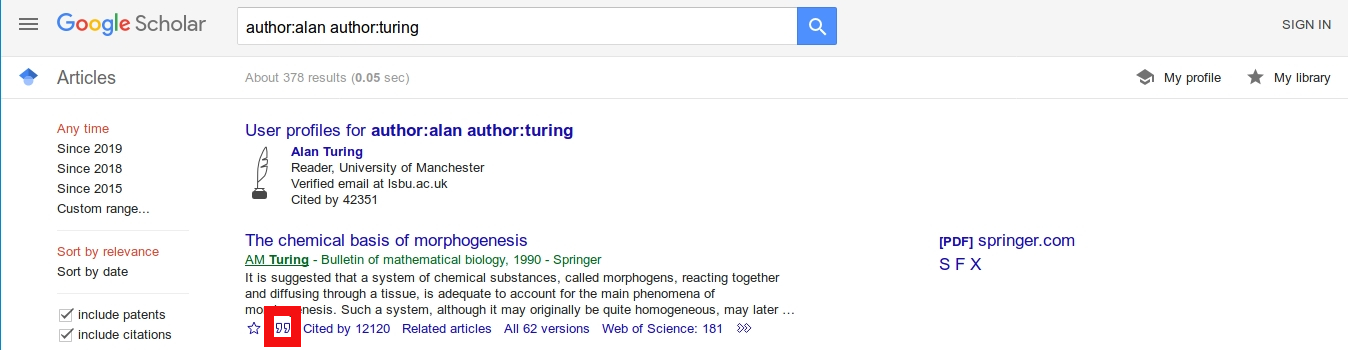
\includegraphics[width=\textwidth]{graphics/google_bibtex1.jpg}  
  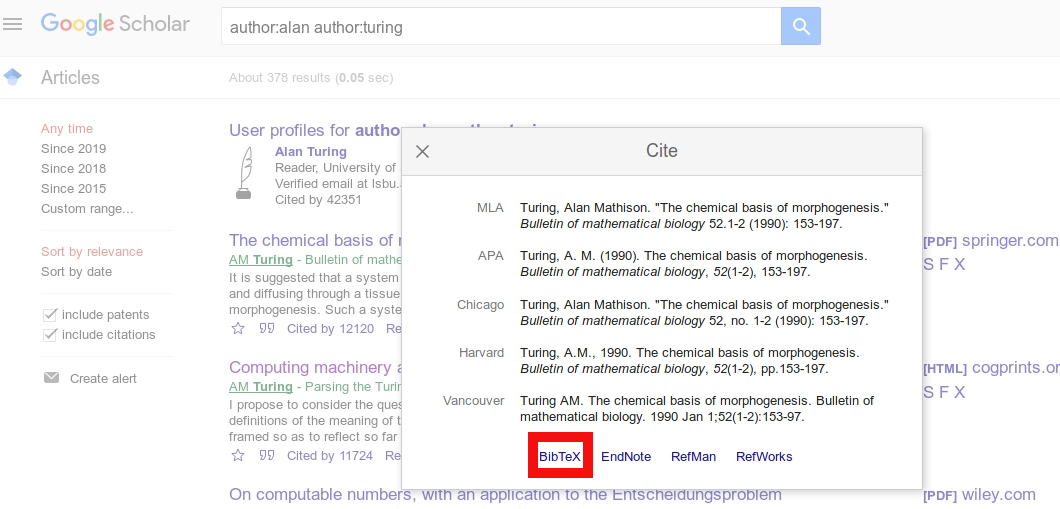
\includegraphics[width=\textwidth]{graphics/google_bibtex2.jpg}  
  \caption{BibTeX-Einträge in Google Scholar abrufen}
  \label{fig:google-scholar-bibtex}
\end{figure}

\subsection{Zitieren}
Durch BibTeX wird LaTeX um einige Befehle (vgl. \cref{tab:bibtex-commands}) zum Zitieren erweitert. 
Zusätzlich benötigt wird das Paket \mintinline{latex}{natbib}.

\begin{table}[H]
  \centering
  \begin{tabular}{ll}
  \toprule
  Funktion                 & Befehl \\ \midrule
  Quelle zitieren          & \mintinline{latex}{\cite{<quelle>}} \\
  Seite zitieren           & \mintinline{latex}{\cite[S. 15]{<quelle>}} \\
  Weitere Zusätze zitieren & \mintinline{latex}{\cite[<präfix>][<suffix>]{<quelle>}} \\
  .bib-Datei einbinden     & \mintinline{latex}{\bibliography{<.bib-datei>}} \\
  Zitierstil ändern        & \mintinline{latex}{\bibliographystyle{<zitierstil>}} \\ \bottomrule
  \end{tabular}
  \caption{Befehle zum Zitieren von Literatur}
  \label{tab:bibtex-commands}
\end{table}

Als \mintinline{latex}{<quelle>} wird immer der BibTeX-Key angegeben.
Verfügbare Zitierstile\footnote{Vollständigere Liste: \url{https://www.overleaf.com/learn/latex/Biblatex_citation_styles}} sind zum Beispiel alpha, natdin und apa.

\section{Ausblick}

Natürlich konnten wir euch in diesem knappen Rahmen nicht ansatzweise zeigen, was \LaTeX{} alles zu bieten hat.
In diesem letzten Abschnitt haben wir daher ein paar Informationen gesammelt, die euch dabei helfen sollen, selbständig tiefer einzusteigen.

\subsection{Pakete}

Einige Pakete haben wir euch bereits vorgestellt, es gibt aber noch ein paar tausend weitere.
Für einige häufig benötigte Features haben wir euch hier eine kurze Liste passender Pakete zusammengestellt:

\begin{figure}[p]
	\widebox{
		% Top rules:
		\colrules
		% Left content: code listing:
		\begin{subfigure}{\widefigurewidth}
			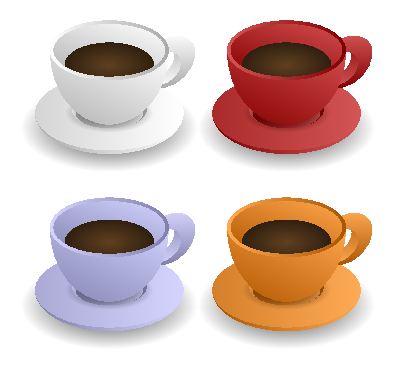
\includegraphics[width=\linewidth]{graphics/coffee-cup.pdf}
		\end{subfigure}
		\hspace{\widefiguregap}
		% Right content: image or rendered example:
		\begin{subfigure}{\widefigurewidth}
			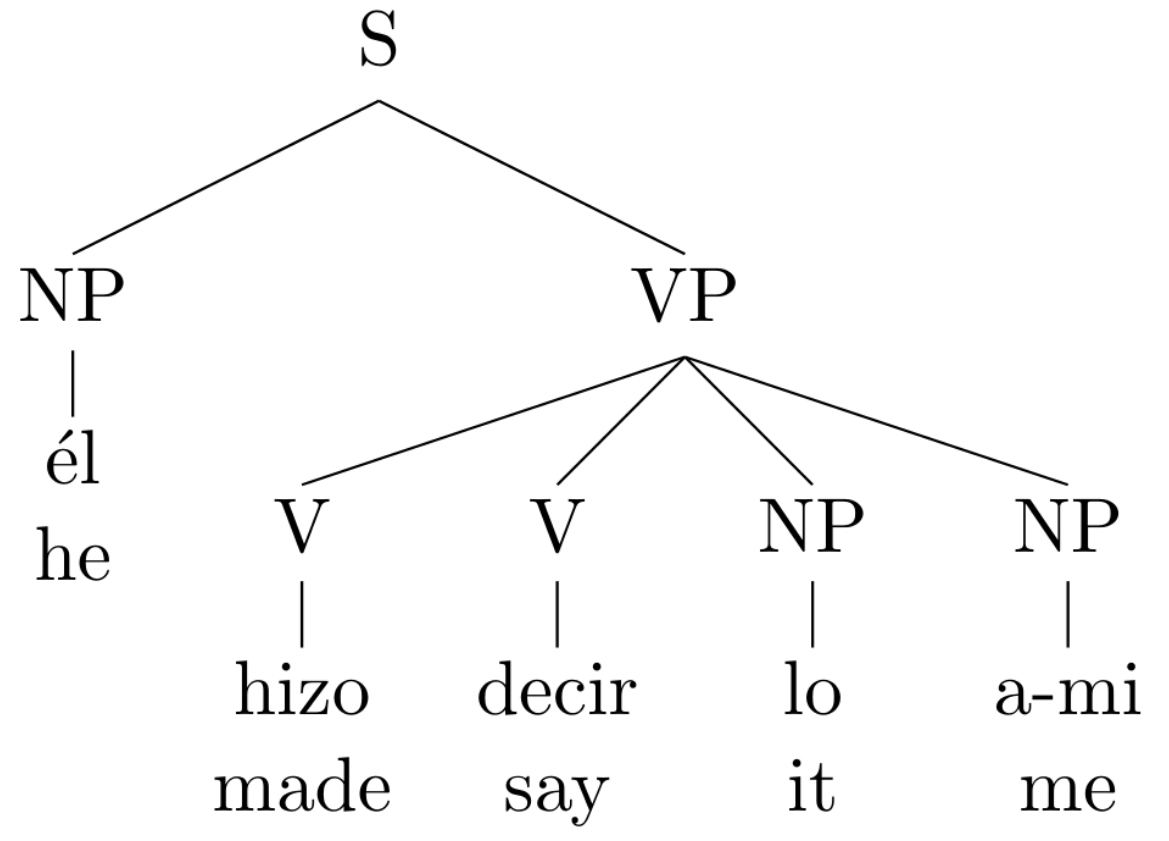
\includegraphics[width=\linewidth]{graphics/qtree.png}
		\end{subfigure}
		% Bottom rules:
		\colrules
		% Left caption:
		\begin{subfigure}[t]{\widefigurewidth}
			\caption{Vektorgrafiken mit TikZ}
			\centering\tiny{\url{https://texample.net/tikz/examples/coffee-cup/}}
			\label{fig:tikz-example}
		\end{subfigure}
		\hspace{\widefiguregap}
		% Right caption:
		\begin{subfigure}[t]{\widefigurewidth}
			\caption{Konstituentenbäume mit qtree}
			\centering\tiny{\url{https://www.ling.upenn.edu/advice/latex/qtree/}}
			\label{fig:qtree-example}
		\end{subfigure}
		\medskip

		% Top rules:
		\colrules
		% Left content: code listing:
		\begin{subfigure}{\widefigurewidth}
			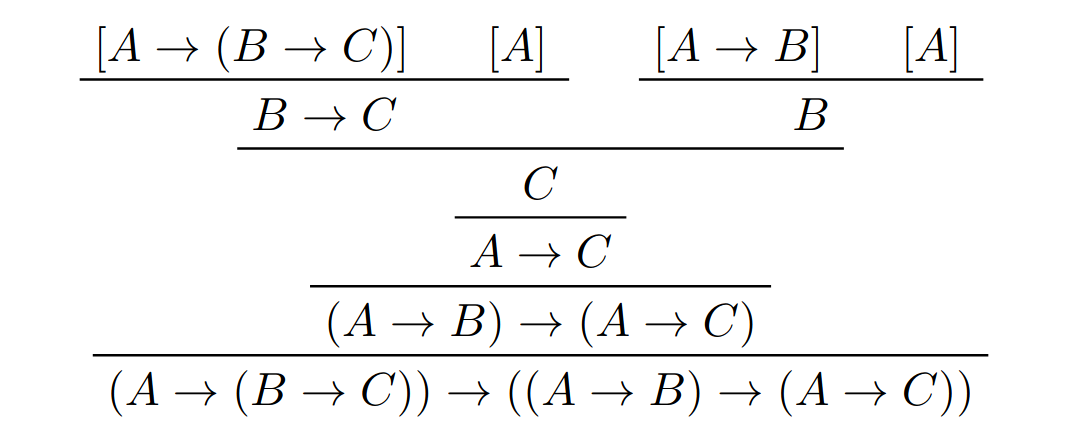
\includegraphics[width=\linewidth]{graphics/prftree.png}
		\end{subfigure}
		\hspace{\widefiguregap}
		% Right content: image or rendered example:
		\begin{subfigure}{\widefigurewidth}
			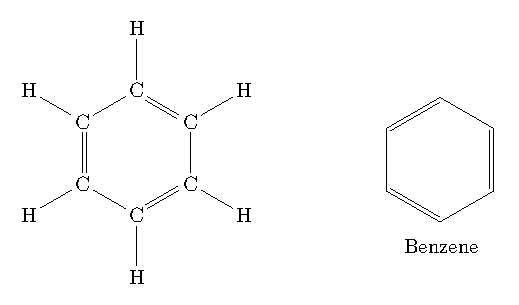
\includegraphics[width=\linewidth]{graphics/benzene-ring.pdf}
		\end{subfigure}
		% Bottom rules:
		\colrules
		% Left caption:
		\begin{subfigure}[t]{\widefigurewidth}
			\caption{Beweisbäume mit prftree}
			\centering\tiny{\url{https://ftp.gwdg.de/pub/ctan/macros/latex/contrib/prftree/}}
			\label{fig:prftree-example}
		\end{subfigure}
		\hspace{\widefiguregap}
		% Right caption:
		\begin{subfigure}[t]{\widefigurewidth}
			\caption{Chemische Strukturformeln mit chemfig}
			\centering\tiny{\url{http://latex-cookbook.net/cookbook/examples/benzene-ring/}}
			\label{fig:chemfig-example}
		\end{subfigure}
		\medskip
	}
	% General caption:
	\caption{Beispiele zu verschiedenen Paketen}
	\label{paket-beispiele}
\end{figure}


\begin{description}
	\item[Stichwortverzeichnisse]
		können mit \texttt{makeidx} automatisiert erstellt werden.\footnote{\url{https://www.ctan.org/pkg/makeidx}}
		Mit \mintinline{tex}{\index{…}} werden im Text einzelne Stichwörter ausgezeichnet, \mintinline{tex}{\printindex} sammelt sie in einem Verzeichnis mit Referenzen.
	\item[Vektorgrafiken]
		(\cref{fig:tikz-example})
		lassen sich mit \texttt{TikZ} (rekursives Akronym für \emph{TikZ ist kein Zeichenprogramm}) direkt im \LaTeX{}-Code erstellen.\footnote{\url{https://www.ctan.org/pkg/pgf}}
		Achtung: Dieses Paket ist sehr mächtig, aber nicht unbedingt einsteigerfreundlich.
		Bevor ihr damit etwas von Grund auf selbst gestaltet, empfehlen wir euch, mit einigen der Beispiele bei \TeX{}ample\footnote{\url{https://texample.net/tikz/examples/}} zu experimentieren.
		Für bestimmte Anwendungsfälle gibt es aber auch spezielle Pakete, die dann meist einfacher zu handhaben sind:
	\item[Konstituentenbäume,]
		die Sätze in ihre grammatikalischen Bestandteile zerlegen (\cref{fig:qtree-example}), erzeugt \texttt{qtree}.\footnote{\url{https://ctan.org/pkg/qtree}}
	\item[Beweisbäume,]
		wie sie in der Logik benötigt werden (\cref{fig:prftree-example}), erzeugt \texttt{prftree}.\footnote{\url{https://www.ctan.org/pkg/prftree}}
	\item[Chemische Strukturformeln]
		(\cref{fig:chemfig-example})
		können unter anderem mit \texttt{chemfig} erzeugt werden.\footnote{\url{https://www.ctan.org/pkg/chemfig}}
	\item[Farbe]
		bringt \texttt{xcolor} in eure Dokumente.\footnote{\url{https://www.ctan.org/pkg/xcolor}}
	\item[Notizen,]
		die ihr bei der Abgabe garantiert nicht überseht, fügt \texttt{todonotes} ein.\footnote{\url{https://www.ctan.org/pkg/todonotes}}
		Damit könnt ihr markieren, was ihr noch \todo{Nicht ändern, das ist ein Beispiel.}ändern oder einfügen wollt.
	\item[Seiten aus anderen \acro{PDF}-Dateien]
		integriert ihr mit \texttt{pdfpages}.\footnote{\url{https://www.ctan.org/pkg/pdfpages}}
		Das eignet sich sehr gut, um Ausgaben anderer Programme in eure Arbeit zu integrieren, beispielsweise in einem Anhang. 
		Einmal kompilieren, und schon ist auch der Anhang wieder auf dem neuesten Stand, wenn das externe Programm etwas geändert hat.
	\item[Verschachtelte Abbildungen]
		und die nahezu beliebige Positionierung von Bildunterschriften ermöglicht \texttt{subcaption}.\footnote{\url{https://www.ctan.org/pkg/subcaption}}
		Davon haben wir auch in diesem Dokument ausgiebig Gebrauch gemacht.
	\item[Tabellen]
		können noch sehr viel flexibler gestaltet werden, als wir es hier gezeigt haben.
		Dabei helfen unter anderem die Pakete 
		\todo{War da die Länge des Namens das entscheidende Auswahlkriterium? :D}
		\texttt{colortbl},\footnote{\url{https://www.ctan.org/pkg/colortbl}}
		\texttt{tabularx},\footnote{\url{https://www.ctan.org/pkg/tabularx}}
		\texttt{multirow},\footnote{\url{https://www.ctan.org/pkg/multirow}}
		\texttt{makecell}.\footnote{\url{https://www.ctan.org/pkg/makecell}}
\end{description}

\noindent Eigentlich kein Paket, sondern eine weitere Dokumentenklasse ist \textbf{beamer:} Damit könnt ihr \textbf{Bildschirmpräsentationen} mit \LaTeX erstellen.
Informationen und Beispiele dazu gibt es bei Overleaf\footnote{\url{https://www.overleaf.com/learn/latex/Beamer}} –
womit wir schon beim nächsten Abschnitt sind:

\subsection{Hilfe und Informationen}

Eine deutlich ausführlichere Einführung in \LaTeX{} bietet \textbf{Wikibooks.}
Das deutschsprachige Wikibook\footnote{\url{https://de.wikibooks.org/wiki/LaTeX-Kompendium}} ist dabei noch etwas unvollständiger als das englischsprachige.\footnote{\url{https://en.wikibooks.org/wiki/LaTeX}}
Beide verweisen bei Bedarf auf zusätzliche Pakete.

Falls ihr mehr Informationen zu einem bestimmten Paket sucht, ist \acro{\textbf{CTAN}}\footnote{\url{https://ctan.org/}} die zentrale Anlaufstelle.
Dort findet ihr zu jedem Paket die offizielle Dokumentation als \acro{PDF}-Dokument.
Darin sind vor allem die ersten Abschnitte interessant, weiter hinten folgen Implementierungsdetails, die ihr normalerweise nicht braucht.

Wenn die Dokumentation zu theoretisch ist und ihr auf der Suche nach praktischen Beispielen seid, kann \textbf{Overleaf}\footnote{\url{https://www.overleaf.com/}} weiterhelfen.
Das primär ein kollaborativer Online-\LaTeX-Editor, ihr findet dort aber auch einige Vorlagen\footnote{\url{https://www.overleaf.com/latex/templates}} für verschiedene Arten von Dokumenten (Lebensläufe, Abschlussarbeiten u.\,v.\,m.).
Speziell zu TikZ bietet \textbf{\TeX{}ample}\footnote{\url{https://texample.net/}} eine Vielzahl an Beispielen.

Bei konkreten Fragen oder Problemen hilft – wie üblich – die Frage-Antwort-Plattform \textbf{Stackexchange} weiter:
Es gibt dort auch eine \TeX-Community.\footnote{\url{https://tex.stackexchange.com/}}

Und selbstverständlich könnt ihr euch auch immer gerne uns wenden:
per Mail an \href{mailto:fachschaft-wiai.stuve@uni-bamberg.de}{fachschaft-wiai.stuve@uni-bamberg.de}, telefonisch unter 0951\,963\,1219 oder in unserem Büro in WE5/02.104.



% References

\end{document}
